% 3 TraceAssist -- 1.75 pages (incl. Fig. 1, full width)
\section{TraceAssist}
\label{sec:traceassist}

\begin{figure*}[t]
\centering
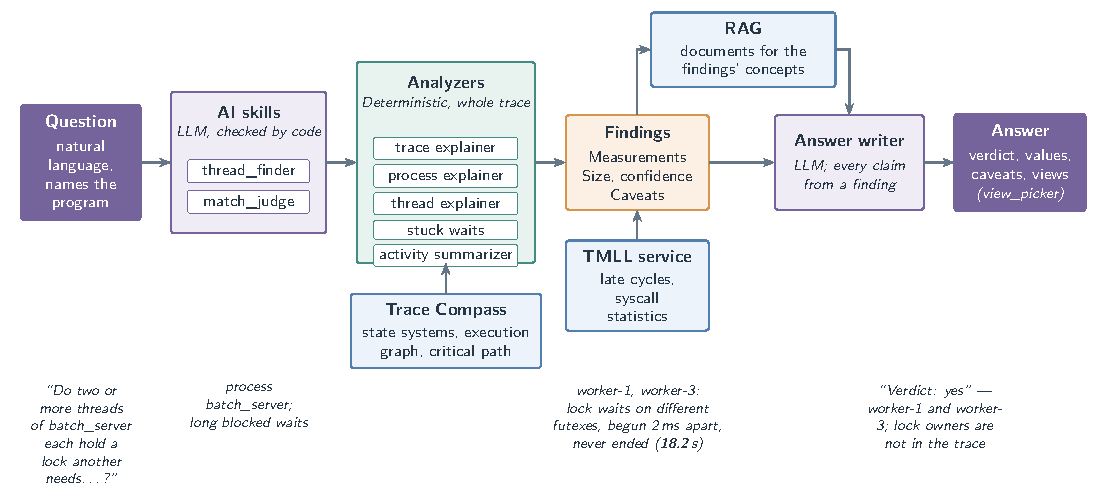
\includegraphics[width=\textwidth]{traceassist_pipeline}
\Description{Flow diagram: question, AI skills, analyzers over Trace Compass, findings with TMLL and RAG, answer writer, answer; with a deadlock question traced through each step.}
\caption{\sysname's pipeline from question to answer. Code computes every fact about the trace; the LLM makes small, checked decisions (the AI skills) and writes the answer from the findings. The italic text follows one bench question, on a trace where two of \texttt{batch\_server}'s workers deadlock, through the steps (Section~\ref{sec:results}).}
\label{fig:pipeline}
\end{figure*}

\sysname follows one rule: \emph{code computes every fact about the trace, and the LLM only makes small, checked decisions and writes the answer from those facts}. A 30-second trace of a small program on a desktop holds 1.4--25 million events (Section~\ref{sec:bench}); the LLM never reads them. It receives about 10--30 thousand tokens of computed evidence per question. Fig.~\ref{fig:pipeline} shows the parts, which we describe in the order a question passes through them; Fig.~\ref{fig:arch} shows the full architecture, drawn on TMLL's architecture figure~\cite{shahedi2025tmll}, with the components we added marked NEW.

\begin{figure*}[t]
\centering
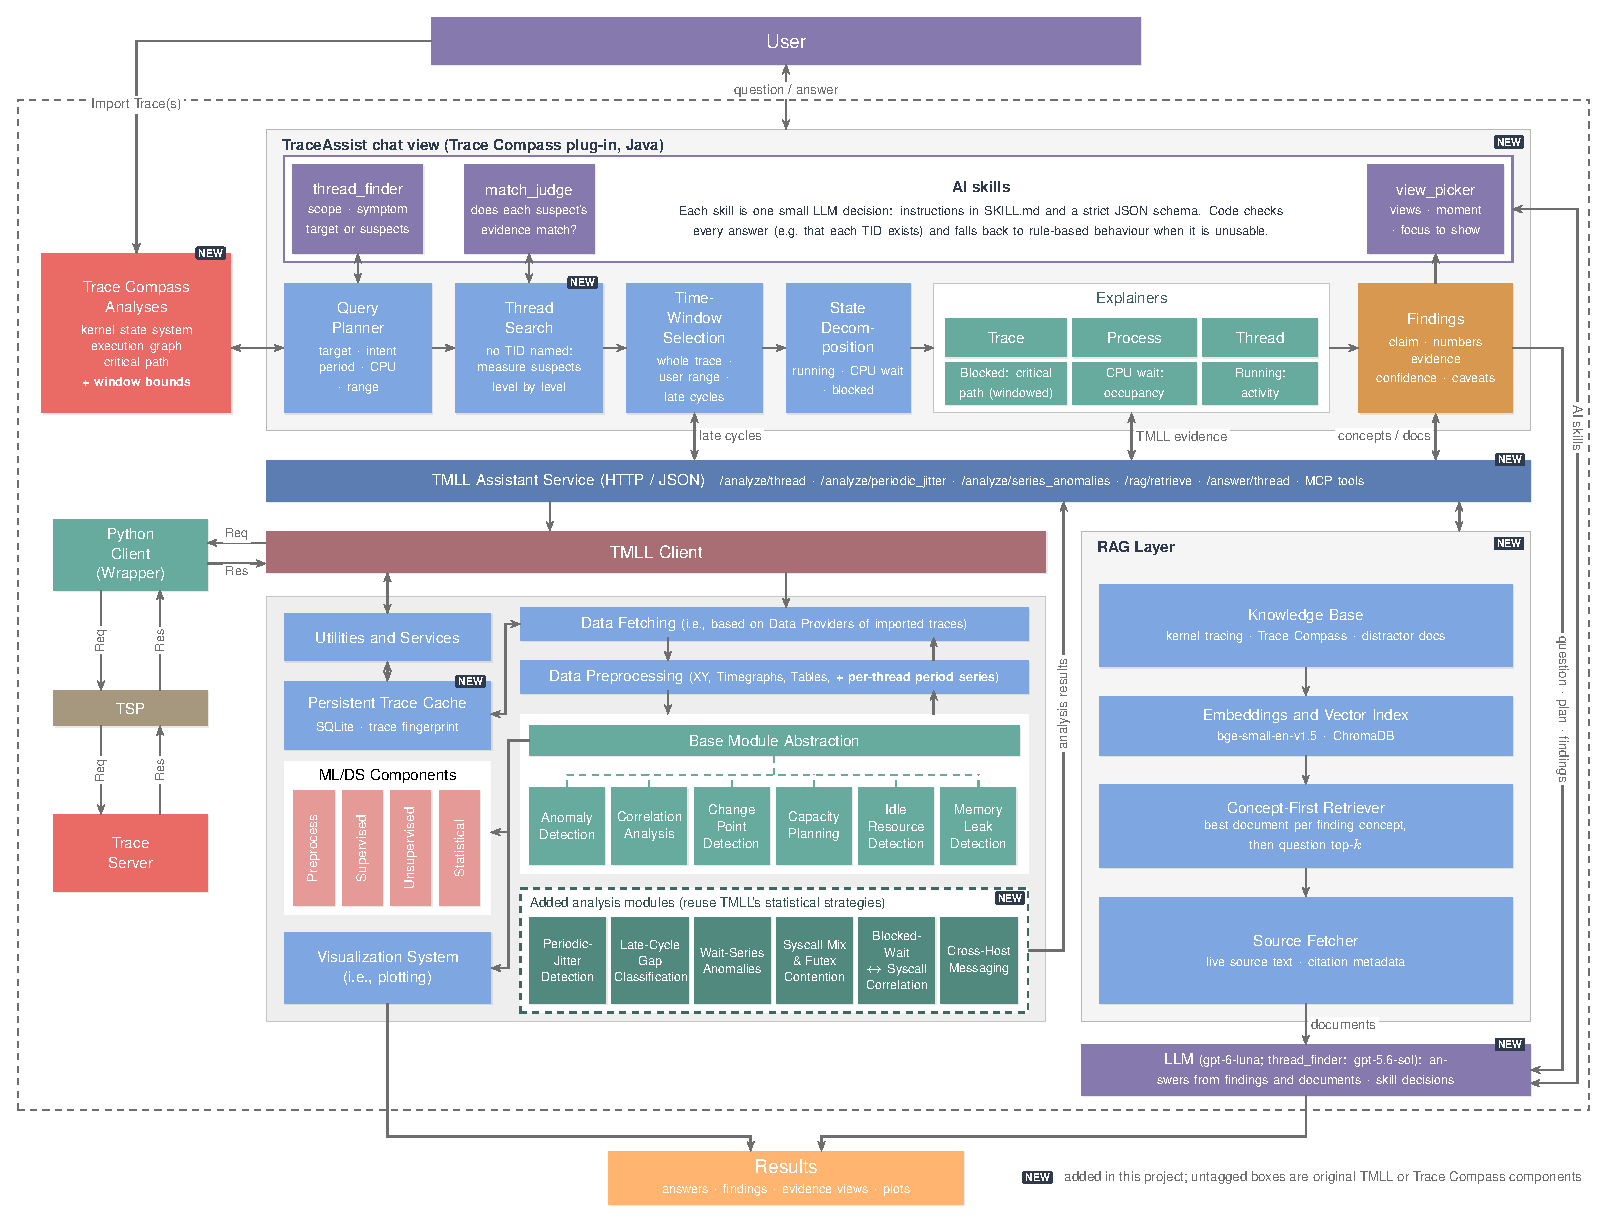
\includegraphics[width=\textwidth]{architecture}
\Description{Architecture diagram of TraceAssist inside Trace Compass, the TMLL assistant service and client with added analysis modules, the RAG layer and the LLM, with new components marked.}
\caption{\sysname's architecture, drawn on TMLL's architecture figure. Boxes marked NEW were added in this work; the others are original TMLL or Trace Compass components. The AI skills (top row) and the LLM are the only calls to a language model; code checks every skill's answer.}
\label{fig:arch}
\end{figure*}

\subsection{From Question to Target}

Users rarely know thread IDs. They ask \emph{``Is something in batch\_server holding a lock too long?''} The first step decides what the question is about: one thread, a process, or the whole trace; what it asks (explain a thread's time, find a process's bottleneck, find late cycles); and the time window. This step needs language understanding most, so it is handed to the first of three \emph{AI skills}.

An AI skill is one narrow decision delegated to an LLM, defined by an instruction file and a strict JSON schema, and checked by code before use:
\begin{itemize}
  \item \textbf{thread\_finder} reads the question and an inventory of the trace's processes and threads, and returns the scope, the symptom the question describes (e.g., a one-off delay or a bottleneck), and either the target or up to five suspects. Every TID and PID it names must exist in the trace; if the call fails, a rule-based planner takes over.
  \item \textbf{match\_judge} rates suspects during the \emph{thread search}. When the target is unclear, code measures every suspect one level deeper at a time (time by state, then the symptom's detail, then the worst moment), and after each level the skill rates whether each suspect's measured evidence matches the question. Code turns the ratings into a pick with a percentage and a confidence label, which the answer reports.
  \item \textbf{view\_picker} chooses the 1--3 Trace Compass views that show the answer's evidence, the moment to show, and what to select in each, from one description file per view. Code computes the zoom range.
\end{itemize}
Skills can be read and changed without touching the Java code. In normal use their decisions are cached per input, so a repeated question gets the same target.

\subsection{Analyzers and Findings}

The analyzers are Java code inside Trace Compass. They read its kernel analyses: the \emph{state system}, which holds each thread's state, current system call and each CPU's run queue over time, and the \emph{execution graph}, which records which thread woke which. There is one analyzer per kind of target:
\begin{itemize}
  \item The \emph{trace explainer} summarizes what was recorded: which events, which processes ran and used the CPU, and which process is the workload rather than background activity or the tracer.
  \item The \emph{process explainer} splits each thread's time into running, waiting for a CPU and blocked; follows the execution graph's wake-up edges to find which thread ended each wait; and names the \emph{bottleneck}, the thread the main thread waits on, with its wait chain to the root. Over every round it measures when each thread finishes and how much faster rounds would be without the bottleneck's wait.
  \item The \emph{thread explainer} splits one thread's time by state and explains each large share: for blocked time, the system call and the critical path~\cite{giraldeau2016wait} of the longest wait; for CPU waits, which threads held the CPU; for running time, user versus kernel time.
\end{itemize}
Trace Compass computes a critical path over a thread's whole life; we added an optional time window so that it can cover one wait, such as the longest. This is the only change to Trace Compass itself.

Two further components cover what the state system does not keep; the first was added, and the second extended, when the evaluation exposed gaps (Section~\ref{sec:lessons}). \emph{Stuck-wait detection} reports threads still blocked at the end of the trace, which the execution graph omits because they are never woken, and classifies their system calls as sleeps, timed waits or waits that only another thread can end; several lock-style waits beginning together are reported, hedged, as consistent with a deadlock. The \emph{activity summarizer} reads every event once and records what the state system does not keep: which file, socket or pipe each call used, open modes, syncs and their durations, threads and processes created and how they ended, and each thread's time in system calls by what they wait on (storage, network, futex, sleep, and so on).

Every result is a \emph{finding}: a JSON object with a one-sentence claim whose numbers are filled in by code, the window it covers, the evidence, a confidence level and caveats. Inferences a kernel trace cannot observe directly, such as which thread holds a lock, are marked medium confidence. Findings also carry their \emph{size}: a bottleneck's impact on the round is labelled negligible (under 5\%), minor or significant (25\% or more), and scheduling delays are counted by length. In a healthy program some thread always finishes last and some wait is always the longest; without sizes, the answer writer reported those as problems.

\subsection{Statistical Evidence and Documentation}

\textbf{TMLL and our modules.} TMLL~\cite{shahedi2025tmll} is the Trace Compass project's machine-learning library. It fetches the Trace Server's analyses through the Trace Server Protocol and applies ready-made modules, such as anomaly detection, change points, correlation, idle resources, capacity planning and memory leaks, to system-wide series such as CPU, memory and disk usage. We keep the library unchanged and built our own components on it (marked NEW in Fig.~\ref{fig:arch}). They analyze one thread's series rather than the whole system, reusing TMLL's statistical strategies:
\begin{itemize}
  \item a \emph{system-call frequency} module, which counts each thread's calls by name and category, classifies the dominant kind (file I/O, synchronization, networking, and so on), and measures futex contention;
  \item per-thread \emph{anomaly detection}: periodic-jitter detection over the intervals between a thread's wake-ups, which finds its late cycles with TMLL's z-score strategy; classification of what the thread was doing during each late cycle; and a wait-series detector that tells a constant slowdown, where every round waits alike, from occasional spikes;
  \item correlation of long blocked waits with the system calls that overlapped them, and detection of messages between hosts.
\end{itemize}
A local HTTP service exposes these to the Java analyzers, and a persistent cache keyed by the trace's fingerprint scans each trace's tables once. We also fixed TMLL's z-score preprocessing, which dropped every value tied at the minimum and so found nothing on a very regular periodic thread. Results return as findings. The service is optional: when it fails, \sysname records an ``unavailable'' finding and the analyzers' findings are unchanged.

\textbf{RAG.} The knowledge base holds 37 Markdown documents: 15 on Linux kernel tracing concepts (futex waits, thread states, wake-ups, system calls), 12 on Trace Compass analyses and their limits, and 10 on Django from an unrelated workload. Documents are embedded with \texttt{bge-small-en-v1.5}~\cite{xiao2023cpack} and stored in ChromaDB. Retrieval is driven by the findings: each concept a finding names, such as the system call a thread blocked in, retrieves its best document, and the question's own search fills the remaining places, six in all. Documents explain concepts; they are never a source of facts about the trace.

\subsection{Answer Writer}

One LLM call writes the answer from a JSON object holding the question, the plan, the findings and the documents. Its rules require that every statement about the trace come from a finding, with its numbers; that no cause, thread or duration be added that no finding states; that missing evidence be stated rather than guessed; that medium-confidence findings be presented as likely; and that a question of the form ``is X happening?'' be decided by the size of the evidence against the question's threshold, so that a minor bottleneck or a handful of delays among thousands does not count. The answer starts with the target the thread search picked, if any, and ends with the views to open.

All LLM calls use OpenAI's \texttt{gpt-6-luna}, except thread\_finder, which uses the larger \texttt{gpt-5.6-sol} at temperature~0. Choosing the threads a question means is the most complex decision in the pipeline, and on a smaller question set used in development, the smaller \texttt{gpt-5.6-luna} picked the wrong threads too often.

\subsection{Integration in Trace Compass}
\label{sec:deployment}

\begin{figure*}[t]
\centering
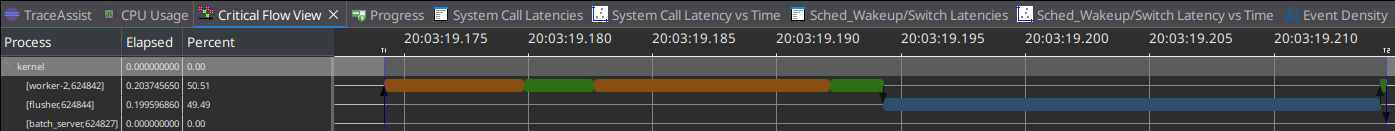
\includegraphics[width=\textwidth]{critical_path_holder_sleeps}
\Description{Screenshot of Trace Compass's critical path view: worker-2 alternates between waiting for a CPU and running, then flusher sleeps on a timer for about 20 ms before worker-2 finishes.}
\caption{The Critical Path view that \sysname opened for \emph{``What is batch\_server's main thread waiting on in each round, and what is holding that up?''} on the bench's lock-holder-sleeps trace, zoomed to one typical 40.3\,ms round. The main thread's wait runs through \texttt{worker-2} (orange: waiting for a CPU while the other workers run; green: running) and then \texttt{flusher}, asleep on a timer (blue) for 19.9\,ms while holding the lock \texttt{worker-2} needs. The answer reported this chain with per-round values within 0.1\,ms of the program's own measurements: \texttt{worker-2} blocked 23.17\,ms per round (measured 23.18\,ms), the lock held 40.13\,ms (40.12\,ms), over all 484 rounds.}
\label{fig:critpath}
\end{figure*}

\textbf{Answers that point to their evidence.} An engineer should not have to trust the answer. Every answer ends with the Trace Compass views that show its evidence, chosen by view\_picker: which views, which moment (the worst wait, a typical round, a late cycle, or the whole trace), what to select in each, and what to look for (Fig.~\ref{fig:critpath}). \sysname then opens these views itself, zoomed to that moment, including a Critical Path computed for the wait in question. The engineer checks the claim in the standard view they already know, and continues the analysis from there.

\sysname is a Trace Compass plug-in: questions are asked in a chat view next to the trace, and the answer streams into it. The pipeline itself has no user interface, so the same code also runs headless in the Trace Compass Trace Server; the evaluation asks its questions there. On 60 test questions, the two chose identical targets and findings.

\textbf{Implementation.} \sysname is about 16{,}600 lines of Java in one Trace Compass plug-in, about 3{,}800 lines of Python for the TMLL modules and the RAG layer, three skill files and 13 view descriptions. The only change to Trace Compass is the critical-path time window. The bench adds about 2{,}100 lines of C for the nine programs and 1{,}700 lines of Python and shell to record the traces, generate the questions and pairs, and score the answers.
